\documentclass[12pt]{article}
\usepackage{settings}

\title{Interactive maps as a tool for visualising multimodal location-based accessibility}
\author{Eemil Haapanen}

\begin{document}
\maketitle

\section{Introduction}
% What accessibility?
The term accessibility is central to this thesis.
Alone, the word simply refers to how easy it is to access something,
with all further meaning derived from
additional explanations and the context in which the word is used.
In this thesis, when referring to accessibility,
I more specifically mean spatial accessibility,
that is, the ease of accessing geographical locations in physical space.

% Geographical accessibility as a phenomenon in general, hard to measure
In this geographical sense,
the general starting point for defining accessibility is often
\enquote{potential of opportunities for interaction} \parencite{han1959}.  % define interaction in more detail?
Depending on the factors considered impactful to that potential,
more precise definitions and measurements can be constructed in many different ways
\parencite{pap2016}.
Even if just using travel distance or time as a measure of access,
including all the different things it can be measured in relation to
would make the amount of variations, i.e. different "accessibilities",
to measure grow exponentially \parencite{lev2020}.
In addition, accessibility is inherently tied not only to location
but also time \parencite{jar2018},
meaning every place in every time has a level of access
in relation to every other place \parencite{lev2020}.
All this makes measuring accessibility in a holistic way a complicated task.

% hard to visualise too
Similarily to defining or measuring it, visualising accessibility is complex.
Accessibility visualisations are often constrained to displaying access in relation to
a limited number of pre-selected places (for example \textcite{wei2018}),
or composing an accessibility index that can be calculated and mapped for all locations,
in relation to potentially many different things and locations (for example \textcite{kim2019}).
However, more complex accessibility measures tend to lead to
less usable presentations \parencite{te2014},
while mapping more simple measures could lead to an influx of variations to present.
For example separating different travel modes, times of day or target locations
would multiply the amount of visualisations needed to present accessibility.

% Not only methodological but also a cartographical challenge 
% something that is not a physical feature nor an easily explainable variable
% ----------------------------------------
% general stuff about cartography - what types of phenomena / maps
% how is accessibility different?
% ----------------------------------------
% Why is visualising access important?
% This could be before the preceding chapter too?
% Leave something for background chapter too

% how interactivity benefits accessibility visualisation (because of how accesibility is)
Even if visualising every aspect of accessibility from everywhere to everywhere is impossible,
interactive visualisations could offer some benefits for presenting accessibility.
After all, a key principle of interactivity in map presentations is
the map user's ability to change the content of the map \parencite{rot2013b}.
For visualising accessibility this could mean, for example,
interactive selection of location or travel mode instead of
a static accessibility index that, to a varying extent, tries to account for everything.
Scientific literature on the topic seems to support the idea of
interactivity in accessibility visualisation, even indicating a need for such presentations.
In a study focusing on the usablity of different accessibility instruments and visualisations,  % accessibility instrument
\textcite{te2014} highlight the importance of real-time interactivity between the map and the map user.
\textcite{but2018} state that for maps to efficiently communicate accessibility,
they should be as flexible and dynamic as possible.
However, \textcite{but2018} also note that these qualities are often missing in accessibility visualisations.
Along the same lines, \textcite{paj2021} find modern accessibility visualisations often complicated,
and lacking in interactivity and flexibility.

% research questions
% Communicating accessibility instead of analyzing it
% How to utilize interactive mapping in communicating accessibility
This thesis approaches accessibility from a cartographical angle,
especially in the context of interactive mapping.
There are three main research questions.
Firstly, how should accessibility be presented cartographically?
To answer this, I will go into detail of what makes accessibility an unique phenomenon,
especially from a cartographical point of view,
and what requirements this places on visual representations of accessibility.
Secondly, what value do interactive visualisations hold in the context of accessibility?
Here I will focus on the general theory of cartography and especially cartographic interaction,
also previewing previous interactive maps and presentations relative to the topic.
Thirdly, how should an interactive accessibility presentation be implemented?
The goal here is to develop an interactive web-based presentation of the
Helsinki Region Travel Time Matrix \parencite{ten2020}.
In addition to the insights gained from the previous research questions,
I will utilize an iterative development process with interviews
to keep in touch with the map user's perspective.


\section{Background}
A general comprehension of research in both cartography and accessibility is
vital to approaching any of the research questions presented.
In this section I will cover some key themes and advancements in both fields, % advancements?
later relating them more precisely to accessibility visualisations.

% Currently I see the first two research questions as a sort of a background study
% necessary to form a theoretical base
% for the implementation of the interactive matrix visualisation.
% This is why I have placed them in a background section.

% Cartography - How we got to where we are now, what this means for the topic
\subsection{Cartography and maps}

% maps
% basic overview type stuff, relating information to location
% For most of humanity's time maps...
% What cartography, when
Cartography as a dicipline is as dynamic as the topics people map,
or the methods they use to map said topics.
Consequently, the meaning of the word depends hevily on the period in time
during which it is used.
Currently the International Cartography Association defines cartography as
"The science, art, and technology of making and using maps."
\parencite{ica2019}.
Much like cartography, the concept of a map is not static.
For most of humanitys history maps have been a tool to describe the physical world.
Used for navigation and comprehending places.
Nowadays cartography is interlinked with data visualization
Presenting the world (locations) vs presenting data linked to locations (thematic mapping, \parencite{tyn1992})

% To understand how we got to these definitions:
% Change, cartography is different now, 1950-1990
\textcite{mac2004} considers two developments especially important
to understanding how the modern cartographic research has shaped up.

% 1950
The first, set in motion by the second world war, was
the shift from thinking of maps as primarily objects of art and graphic design,
to instead viewing them as scientifically dissectible visual representations
with the primary function of conveying information.
Interlinked with the field of psychology,
functional map design drew from the researh on human perception
in an effort to optimize cartographical methods such as symbology.
The goal of these efforts was finding scientifically provable, "objective", rules
for producing as functional as possible maps.

% 1970
% Cartography as graphic communication.
The second was the change in how a map is thought to work.
Instead of an artifact of it's own knowledge,
a map is essentially just a means to trasnport knowledge in a communication system.
So, the knowledge a map reader gains from reading a map is that of the mapper's,
just disseminated through cartographical communication, i.e. the map.
Thinking this way, no new knowledge is constructed by the map reader,  % TODO check this & debunk later
and the function of cartography can be related to constructing and interpreting messages.
Among the pioneers of this way of thinking about maps was \textcite{kol1969},
who explicitly regarded maps as communication systems.
\textcite{bal1966} graphicacy

However, there have been numerous objections to the paradigm of Cartography as a form of communication.
Firstly, there is the issue of communication versus function:
A mapmaker might not have an intent to communicate any particular message to begin with.

Also, implicit vs explicit:
the message the map reader extracts from a map might differ from the one intended, or


% Moving on from these
Art and science \parencite{mac2004, tyn1992}  % compare these

% 1990
% - More interlinked with GIS
% - critical / qualitative GIS too

% 2010-the present -> interactive
% The change in cartography
Rise of open source \textcite{pet2015}


% The nature of interactive cartography
% More than a map: ui, ux
% What even is an interactive cartographer?
\textcite{rot2013a, rot2013b}


\subsection{Accessibility in the context of cartography}
% This section focuses on the first research question:

% What makes accessibility an unique phenomenon,
% especially from a cartographical point of view,
% and what requirements this places on visual representations of accessibility.

% This will be a litearture review.

% What are the "normal" (cartography-wise) phenomena, do they exist?

\subsection{Interactive maps and their potential in presenting accessibility}
% Interactivity in general
% The default medium for viewing maps and geographical has long been digital.  % TODO add ref
% However, more and more devices allow also for interaction \parencite{mei2019}
The second research question:

\begin{displayquote}
What value do interactive visualisations hold in the context of accessibility?
(General theory of cartography and especially cartographic interaction,
previous interactive maps and presentations relative to the topic.)
\end{displayquote}

Here I will be doing literatrure review as well,
especially relating to the theory of cartography and interactive maps.
Themes such as critical cartography
and the qualitative nature of maps should be found here too.
When previewing previous accessibility visualisations,
some kind of a systematic comparison of previous work
could be a way to form a synthesis here.

\section{Study design}
Describe the study design in more detail.

\section{Data and methods}

This section will focus on the matrix visualisation.

\subsection{Data - Helsinki Region Travel Time Matrix}

General description of the matrix goes here.

\subsection{Methods}

I see the methods necessary to implement the visualisation belonging to two themes:
Methods for figuring out how the map should be
and methods for actually making the map be that way.

For figuring out what the map should be like,
I have (hopefully) at this point already formed some ideas from the background section.
To complement those, and to keep the qualitative aspect of cartography relevant,
interview(s) will be used alongside the development process.

From the technical angle, there are three main components to the map:

\begin{enumerate}
	\item Preprocessing of the matrix to a mappable format
	\item A back-end to serve the matrix
	\item The web map application
\end{enumerate}

See figure \ref{fig:architechture} for my idea of what the architechture might look like.

\begin{figure}[H]
	\centering
	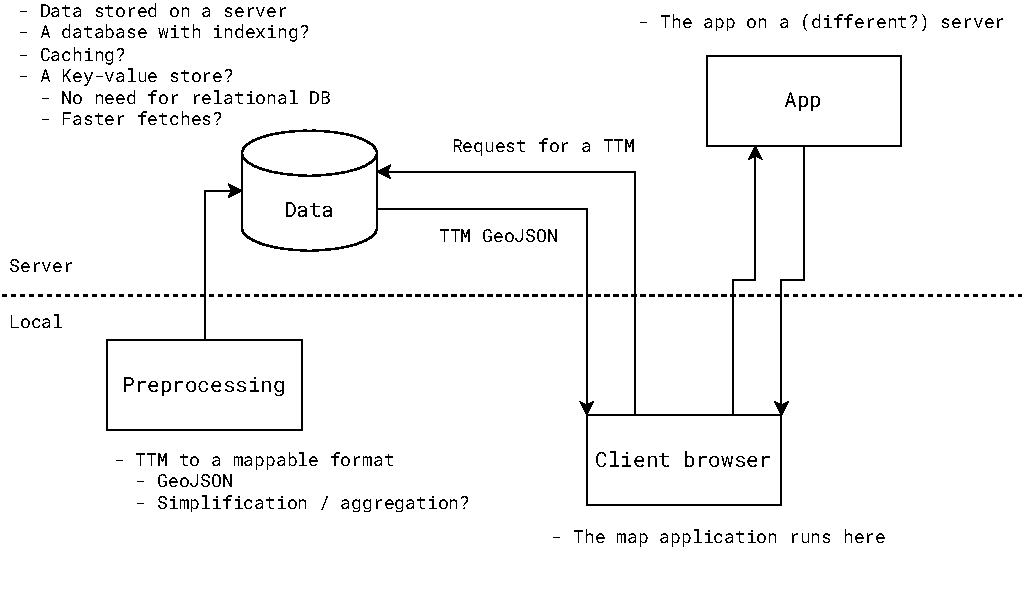
\includegraphics[width=1\textwidth]{images/architechture}
	\caption{Architechture}
	\label{fig:architechture}
\end{figure}

When developing the visualisation, the priority should be on the map application.
However, the development must progress on all components as an iterative process,
where producing a minimal working state should be the first goal.
Something that, to some extent, works, makes discussion about the map possible,
which in turn should keep development progressing towards the right direction.

It should also be noted that the number of techical options for implementing the map is large.
Questions such as which mapping library or UI framework to use,
or how to preprocess the matrix data should be covered here too.
Depending on the need and extent of comparisons between different technologies,
some synthesis could be formed about that too.

\section{Results}

Every research question should have some kind of a result to it.
The first two questions, being more focused on theory rather than implementation,
have their results already in the backround section,
since they are necessary for the rest of the thesis to make sense.
Still, some kind of a synthesis of those results should be here as well.

The results of the implementation of the matrix are, firstly, the visualisation itself,
but also the output of the interviews
and possibly of the technical comparison between technologies.

\section{Discussion}

Discussion and conclusions about the results

\section{Timetable}

I think the work needed to complete this thesis can be divided into three main themes:

\begin{enumerate}
	\item Background study / literature review to gain a theoretical base
	\item Comparing and learning technologies to gain a technical base
	\item The iterative development of the visualisation
\end{enumerate}

My planned timing for the thesis will be from now (summer) to the end of the year (winter).
Even though the themes above will overlap,
my goal is to focus on the first theme first (summer, early fall),
and after that progress towards the last theme (fall, winter).
Realistically, techonogical experimentation will be happening continuously,
but most likely more at the start.

\printbibliography

\end{document}